\documentclass[a4paper, pdftex, 14pt, oneside, titlepage, openany, onecolumn]{book}
\usepackage[spanish]{babel}
\usepackage[utf8]{inputenc}
\usepackage[T1]{fontenc}
\usepackage[pdftex]{graphicx}
\usepackage{makeidx} 
\usepackage{fancyhdr}
\usepackage{listings}
\usepackage{tikz}
\usepackage{setspace}
\newcommand{\HRule}{\rule{\linewidth}{0.5mm}}

\begin{document} 
\pagestyle{fancy}
\renewcommand\headrulewidth{0pt}
\onehalfspace
\lhead{}

\author{Yohan Graterol B.}
\title{NoSQL y MongoDB en Español}
\date{Dic 2013}

\begin{titlepage}
	\begin{center}
		
\includegraphics[scale=0.10]{mongodb}
		\HRule \\[0.4cm]
		{ \huge \bfseries NoSQL y MongoDB en Español \\[0.4cm] }

		\HRule \\[1.5cm]
		
		\begin{minipage}{0.4\textwidth}
			\begin{flushleft} \large
				\emph{Autor:}\\
				Yohan {Graterol B.}
			\end{flushleft}
		\end{minipage}
	    \begin{minipage}{0.4\textwidth}
			\begin{flushright} \large
		%		\emph{Editor:} \\
		%		 
			\end{flushright}
		\end{minipage}

		\vfill

		{\large \today}
	\end{center}
\end{titlepage}

\newpage
\mbox{}
\thispagestyle{empty} 


\vspace*{\fill}
	\begin{flushright} \huge
		A mis padres, hermano y mi novia. 
	\end{flushright}
\vspace*{\fill} 
\chapter*{Prefacio}
\cleardoublepage\makeatletter\@openrightfalse\makeatother 

\tableofcontents

\part{El desconocido NoSQL} 
\chapter{Introducci\'on a NoSQL}

\section{Definici\'on}

NoSQL o "No solamente SQL" ({\bf Not Only SQL}) es un t\'ermino acu\~nado por Carlo Strozzi en 1998 y nuevamente retomado por Eric Evans en 2009 y se refiere a un conjuto de bases de datos que se diferencian en gran parte de las bases de datos convencionales, en caracter\'isticas tanto de uso como de implementaci\'on; estos tipos de bases de datos no usan SQL o al menos no como lenguaje predeterminado para realizar las consultas. Las bases de datos NoSQL (desde ahora "no relacionales"), no soportan totalmente {\bf ACID} \footnote{'ACID: Atomicidad, Coherencia, Aislamiento y Durabilidad'}, esto lo explica el teorema del profesor Eric Brewer, Teorema CAP (2000):

\begin{quote}
Es imposible para un sistema distribuido garantizar simultáneamente las siguientes tres características:

	\begin{itemize}
		\item Consistency (Consistencia): todos los nodos ven la misma data al mismo tiempo.
		\item Availability (Disponibilidad): una garantía de que todos los requerimientos recibirán una respuesta de que el requerimiento fue exitoso o fallido.
		\item Partition Tolerance (Tolerancia a la Partición): el sistema continúa operando a pesar de la pérdida arbitraria de mensajes, o la falla de parte del sistema.
	\end{itemize}
\end{quote}

En primera instancia es una desventaja, pero gracias a esto permite que los motores de bases de datos no relacionales escalen f\'acilmente de manera horizontal. 

El lenguaje SQL no es un lenguaje predominante entre los distintos tipos de bases de datos no relacionales, por lo general cada motor tiene su propio lenguaje de consultas. Cabe destacar que la informaci\'on no se almacena con un esquema fijo (\textbf{pero si usando almacenamiento estructurado}), aun que si existe un esquema que el DBA\footnote{'Database Administrator - Administrador de base de datos'} o el desarrollador propone con anterioridad de manera virtual, es decir, no se crea en el motor antes de utilizar la base de datos sino al almacenar el primer valor.

\section{Tipos de bases de datos no relacionales}

En el mundo de las bases de datos no relacionales nos encontramos con distintos modelos o tipos, que se desempe\~nan mejor en algunos ambientes espec\'ificos; esas distintas facetas no se ven en las base de datos relacionales. En este libro se expondr\'an los tipos m\'as comunes.

\subsection{Bases de datos orientadas a documentos}

Las bases de datos orientadas a documentos o tambi\'en denominadas como {\bf Bases de datos documental}, trabajan bajo el marco de la definici\'on de un \textit{"Documento"}, donde cada motor que usa esta definici\'on difiere en los detalles, pero la mayor\'ia concuerda en como se almacena la informaci\'on con alg\'un formato est\'andar. Los formatos m\'as utilizados por los motores m\'as populares son: {\bf JSON y BSON}. Se podr\'ia  considerar este tipo como el m\'as utilizada en la actualidad.

Cada documento, es muy similar a un registro en una base de datos relacional, donde se puede observar un esquema parecido mas no r\'igido. Dos documentos no tienen porque tener un esquema igual, aunque sean de una misma colecci\'on de datos.

\begin{figure}[!ht]
    \centering
    \begin{lstlisting}
    {
	    _id: 1,
	    nombre: "MongoDB",
	    url: "http://www.mongodb.org",
	    tipo: "Documental"
    }
    \end{lstlisting}
    \caption[Bases de datos documental]{Ejemplo de documento.}
\end{figure}

Este ejemplo demuestra la sencillez de un documento, se observa un modelo al estilo \textit{\textbf{clave : valor}}. Una analog\'ia con las bases de datos relacionales ser\'ia: Clave = Campo y Valor = Dato del campo, hasta all\'i queda la analog\'ia.

\subsection{Bases de datos orientadas a clave/valor}

Este tipo de bases de datos es muy similar a las bases de datos documental en el concepto de guardar la informaci\'on con el modelo clave:valor, la diferencia radica en que un documento se almacena en una clave; esta definici\'on puede parecer algo abstracta. Esto se explica mejor con un ejemplo.

El siguiente ejemplo utiliza el documento de la secci\'on anterior:

\begin{figure}[!ht]
    \centering
    \begin{lstlisting}
    mongodb => {
	    _id: 1,
	    nombre: "MongoDB",
	    url: "http://www.mongodb.org",
	    tipo: "Documental"
    }
    \end{lstlisting}
    \caption[Bases de datos clave/valor]{Ejemplo de un documento en una clave.}
\end{figure}

La clave en este caso es 'mongodb' y su contenido es el mismo documento de la secci\'on anterior. Esto hace que var\'ie la forma de recuperar la informaci\'on con respecto a las bases de datos basadas en documentos.

Algun muy interesante de este tipo es que permite ser utilizado junto bases de datos orientadas a documentos, lo que origina motores h\'ibridos.

\subsection{Bases de datos orientadas a grafos}

Este tipo difiere completamente a los tipos antes mencionados, y trata la informaci\'on de una manera peculiar usando \textbf{grafos}\footnote{Grafo: es un conjunto de objetos llamados nodos unidos por enlaces denotados aristas, que permiten representar relaciones binarias entre elementos de un conjunto.} y \textbf{teor\'ia de grafos}. Cada nodo solo debe contener una sola columna, por lo tanto se debe normalizar completamente las bases de datos. Y como la definici\'on de grafos indica, las relaciones solo pueden ser binarias, es decir, un nodo puede solo usar una relaci\'on para entrar en contacto con otro nodo y no m\'as de uno.

Las ventajas de este tipo de bases de datos van enfocadas a la integridad de los datos, cualquier cambio en un nodo o relaci\'on solo afecta localmente.

\begin{figure}
    \centering
    \begin{tikzpicture}[!ht]
         [scale=.8,auto=left,every node/.style={circle,fill=blue!20}]
         \node (nPedro) at (1,10) {Pedro};
         \node (nJuan) at (4,8)  {Juan};
         \node (nLuis) at (8,9)  {Luis};
         \node (nMaria) at (11,8) {Maria};
         \node (nJulia) at (9,6)  {Julia};
         \node (nYohan) at (5,5)  {Yohan};

         \foreach \from/\to in {nPedro/nJuan,nJuan/nLuis,nLuis/nMaria,nMaria/nJulia,nJulia/nLuis,nJulia/nYohan,nYohan/nJuan}
             \draw (\from) -- (\to);

     \end{tikzpicture}
     \caption[Bases de datos en grafo]{Ejemplo de un gr\'afo con relaciones de conocidos.}
\end{figure}

\section{Sistema de gesti\'on de bases de datos (SGBD)}

Jorge Sánchez Asenjo (2005) define SGBD\footnote{En ingl\'es DBMS: Data Base Management System} como:

\begin{quote}
Un sistema gestor de bases de datos o SGBD es el software que permite a los usuarios procesar, describir, administrar y recuperar los datos almacenados en una base de datos. 
\end{quote}

Un tipo de base de datos no sirve de nada sino tiene un sistema que lo gestione, a menos que desees crear un SGBD. En NoSQL hay una basta gama de SGBD, y la mayor\'ia est\'an bajo licencia de c\'odigo libre, permitiendo as\'i usar, estudiar, modificar y redistribuir sin problema alguno con respecto a algunos motores de bases de datos relacionales con licencias privativas.

\section{Lista de SGBD NoSQL}

\subsection*{Bases de datos documental}

\begin{itemize}
\item MongoDB (Lanzamiento: 2009 / Licencia: GNU AGPL v3.0)
\item CouchDB (Lanzamiento: 2005 / Licencia: Apache License 2.0)
\item Raven DB (Lanzamiento: 2010 / Licencia: GNU AGPL v3.0)
\end{itemize}

\subsection*{Bases de datos clave/valor}

\begin{itemize}
\item Apache Cassandra (Lanzamiento: 2008 / Licencia: Apache License 2.0)
\item Riak (Lanzamiento: 2009 / Licencia: Apache License 2.0)
\item Redis (Lanzamiento: 2009 / Licencia: BSD)
\end{itemize}

\subsection*{Bases de datos en grafos}

\begin{itemize}
\item Neo4j (Lanzamiento: 2009 / Licencia: GNU AGPL v3.0)
\item Dex (Lanzamiento: 2008 / Licencia: Comercial)
\item Sones GraphDB (Lanzamiento: 2012 / Licencia: GNU AGPL v3.0 y comercial)
\end{itemize}

\section{¿Por qu\'e NoSQL?}

En esta \'epoca donde se generan cantidades enormes de datos menos estructurados, las bases de datos relacionales empiezan a mostrar deficiencias, en almacenamiento u operaciones; siendo esta una de las principales razones de impulsar el uso de bases de datos no relacionales. Otras de las razones relevantes es la arquitectura, que permite escalar horizontalmente de manera sencilla sin tantos problemas de rendimiento. \textbf{En cap\'itulos posteriores veremos que es escalamiento horizontal}.

\section{Usos extendidos}

\part{Primeros pasos con MongoDB} 
\chapter{Conociendo MongoDB}

\section{MongoDB}

MongoDB\footnote{MongoDB - http://www.mongodb.org/} es un sistema de bases de datos no relacionales, multiplataforma e inspirada en el tipo de bases de datos documental y clave/valor, su nombre proviene del t\'ermino en ingl\'es "hu\textbf{mongo}us". Est\'a liberada bajo licencia de software libre, espec\'ificamente GNU AGPL 3.0\footnote{AGPL - http://www.gnu.org/licenses/agpl-3.0.html}. MongoDB usa el formato BSON (JSON Compilado) para guardar la informaci\'on, dando la libertad de manejar un esquema libre. Este motor de bases de datos es uno de los m\'as conocidos y usados, pudiendolo comparar en popularidad con MySQL en el caso de las bases de datos relacionales.

El desarrollo de MongoDB comenz\'o en el a\~no 2007 por la empresa 10gen\footnote{10gen - http://www.mongodb.com/}, publicando una version final en el 2009. Para la fecha que es escrito este libro, MongoDB se encuentra en la versi\'on 2.4.8.

\section{T\'erminos b\'asicos entorno a MongoDB}

\subsection{JSON - JavaScript Object Notation}

JSON es formato compacto de representacion de objetos. Las especificaciones las public\'o Douglas Crockford en el documento RFC 4627\footnote{RFC 4627 - http://www.ietf.org/rfc/rfc4627.txt}. JSON es un formato independiente del lenguaje, aunque su uso extendido hasta hace poco era en el lenguaje Javascipt. Actualmente se usa JSON en gran cantidades de sistemas para intercambiar informaci\'ion por su simplicidad en comparaci\'on con XML.

Este formato soporta gran cantidad de tipos de datos, lo que lo hace atractivo para un uso generalizado, y cada vez m\'as lenguajes de programaci\'on dan soporte a este formato. El ejemplo del cap\'itulo anterior, donde se mostraba un "documento", no es m\'as que JSON.

\subsection{Documento}

Un documento es un conjuto de datos estructurados (mas no con un esquema estricto), que contiene pares clave/valor. Un documento puede ser comparado con una fila o registro en una base de datos relacional.

\subsection{Colecci\'on}

Es un conjunto de documentos, similar a una tabla en las bases de datos relacionales.

\section{Instalando MongoDB}

\subsection{Instalaci\'on en Linux desde la fuente}

Existen distintas formas de instalar MongoDB en Linux, una de ellas, y la menos recomendable es compilar el c\'odigo fuente que pueden descargar desde: http://www.mongodb.org/downloads. Tambi\'en se puede descargar los binarios, descomprimirlos y usarlos.

\subsection{Instalaci\'on en Linux desde los repositorios}

Los sistemas Linux a diferencia de otros SO, manejo sus software en repositorios, que no es m\'as que un sitio centralizado donde se almacenan todos los software disponible para una distribuci\'on de Linux.

\subsection*{Instalaci\'on en Fedora Linux, Red Hat Linux Enterprise y Derivados}

Para instalar MongoDB en alguna de estras distribuciones, se debe hacer uso del gestor de paquetes yum y ejecutar el siguiente comando:

\begin{lstlisting}
    yum install mongodb mongodb-server
\end{lstlisting}

\begin{itemize}
    \item \textit{\textbf{mongodb}}: Contiene todos los paquetes ``cliente'', como es el caso del cliente \textbf{mongo}, la herramienta para respaldos en binarios de bases de datos \textbf{mongodump}, \textbf{mongorestore} para recuperar respaldos en binario, \textbf{mongoexport} y \textbf{mongoimport} que realizan una acc\'ion similar a mongodump y mongorestore, pero usan formato JSON o CSV.
    \item \textit{\textbf{mongodb-server}}: Contiene todos los paquetes para hacer funcionar el servidor, como el demonio \textbf{mongod}.
\end{itemize}

mongodb y mongodb-server se pueden instalar independientemente. ?`Cu\'ando hacer eso? Un caso muy representativo es cuando se desea colocar en producci\'on la base de datos. Se recomienda solo instalar los paquetes de servicio mongodb-server y el cliente en otra m\'aquina.

Para iniciar/reiniciar o apagar el demonio de MongoDB en \textbf{Fedora} se utiliza el siguiente comando:

\begin{lstlisting}
    systemctl start|restart|stop mongod.service
\end{lstlisting}

En el caso de \textbf{Red Hat Enterprise Linux 6} o derivados:

\begin{lstlisting}
    service mongod start|restart|stop
\end{lstlisting}

Para activar el inicio de MongoDB en el arranque del sistema debe ejecutar segun sea el caso lo siguiente:

\textbf{Fedora}

\begin{lstlisting}
    systemctl enable mongod.service
\end{lstlisting}

\textbf{Red Hat Enterprise Linux 6} o derivados:

\begin{lstlisting}
    chkconfig mongod on
\end{lstlisting}

\subsection*{Instalaci\'on en Debian}

En el caso de Debian, en un solo paquete se encuentra la distribuci\'on completa de MongoDB y para instalarlo se utiliza el gestor de paquetes apt-get:

\begin{lstlisting}
    apt-get install mongodb
\end{lstlisting}

\subsection*{Instalaci\'on en ArchLinux}

Haciendo uso del gestor de paquetes pacman:

\begin{lstlisting}
    pacman -S mongodb
\end{lstlisting}

\subsection{Instalaci\'on en Mac OS X}

\subsection*{Instalaci\'on Manual}

Puede descargar la \'ultima versi\'on disponible de MongoDB para Mac OS X usando cURL\footnote{cURL es una herramienta para usar en un intérprete de comandos para transferir archivos con sintaxis URL}, descomprimirlo y colocarlo en una carpeta a conveniencia.

\begin{lstlisting}
    curl -O http://downloads.mongodb.org/osx/mongodb-osx-x86_64-XXX.tgz
\end{lstlisting}

Siendo XXX, la versi\'on disponible. Ahora se descomprime el archivo usando la herramienta tar.

\begin{lstlisting}
    tar -zxvf mongodb-osx-x86_64-XXX.tgz
\end{lstlisting}

Con todos los archivos de MongoDB en su Mac OS X, solo debe ingresar a la carpeta resultante y ejecutar el demonio \textbf{mongod}.

\subsection*{Usando Homebrew}

\begin{lstlisting}
    brew update
    brew install mongodb
\end{lstlisting}

\section{La consola interactiva de MongoDB}

Ya con la previa instalaci\'on de MongoDB y sus herramientas, podemos acceder a su consola interactiva y realizar nuestras primeras interacciones con MongoDB.

\begin{figure}[!ht]
    \centering
    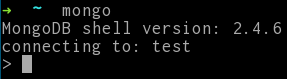
\includegraphics[scale=1]{mongodb_consola} 
    \caption[Consola de MongoDB]{Consola de MongoDB.}
\end{figure}

Al iniciar la consola se conecta autom\'aticamente a la base de datos \textit{\textbf{"test"}}, y apartir de all\'i podemos realizar consultas sobre esa base de datos. La consola es importante para administrar MongoDB, puede parecer desafiante para los que no est\'an acostumbrado a usar herramientas en c\'onsola, pero la gente de 10gen pens\'o en eso y agreg\'o comandos f\'aciles de recordar.

\section{Conectando a bases de datos}

La conexi\'on a bases de datos desde la consola o a trav\'es de alg\'un lenguaje es muy sencillo; a\'un as\'i en MongoDB NO se crean las bases de datos antes de usarla. En bases de datos relacionales, se debe crear toda una estructura inicial para poder almacenar informaci\'on, al menos se debe tener una base de datos con una tabla, eso en MongoDB no se hace. Para crear una base de datos se debe seleccionar, luego almacenar un documento creando una colecci\'on de documentos.

\subsection{Seleccionando la base de datos}

Antes de seleccionar una base de datos, uno tiene la opci\'on de ver el listado de bases de datos que existen en el sistema, con el comando \textit{\textbf{show dbs}}.

\begin{lstlisting}
    > show dbs
    admin	0.203125GB
    fudcon	0.453125GB
    irianas_server	0.203125GB
    irianas_web	0.203125GB
    local	0.078125GB
    mongoengine	0.203125GB
    mongoenginetest	0.203125GB
    mongoenginetest2	0.203125GB
    mongoenginetest4	0.203125GB
    test_files	0.203125GB
\end{lstlisting}

La salida nos muestra el nombre y el tama\~no de la base de datos, es importante mencionar que MongoDB al crear el primer documento reserva espacio en disco.

Luego de saber la lista de bases de datos existente, debo seleccionar una, no es obligatorio que est\'e en la lista, sencillamente haciendo uso del comando \textit{\textbf{use basededatos}}, se selecciona y podemos trabajar con la base de datos existente u operar para crear una nueva.

\begin{lstlisting}
    > use libromongodb
    switched to db libromongodb
\end{lstlisting}
\chapter{CRUD en MongoDB}

\section{?`Qu\'e es CRUD?}

\section{Create}

\section{Read}

\section{Update}

\section{Delete}
\include{capitulo4}
\include{capitulo5}

\backmatter
\include{glosario} 

\printindex
\end{document}